\textit{Примечение:} везде, если не оговорено иное, имеются в виду правые и левые берега рек \textit{орографически}.
\subsection{18 августа. Старт}
\textit{Метеоусловия: утром, днём, вечером ясно, тепло.}

Приезжаем в г. Минеральные Воды в 03:40. Встречаемся на вокзале с участником, прибывшим на день раньше и загружаемся в машину Бориса Саракуева. В 04:00 отправляемся на место старта (мост через р. Учкулан, N 43.38668\degree~E 41.98961\degree), куда прибываем в \alert{СКОЛЬКО?}. Разпределяем заброски, отдаём их водителю и выдвигаемся на маршрут в \alert{СКОЛЬКО?}. Первые 1.5 км до коша проходим по д.р. Учкулан, затем тропа проходит через калитку и поврачивает направо, на подъём в висячую долину р. Кичкинакол Джалпаккольский.

\begin{figure}[h]
	\centering
	\includegraphics[width=0.7\linewidth]{../pics/DSC_0412}
	\caption{группа на старте маршрута в д.р. Учкулан}
	\label{fig:uchkulan}
\end{figure}


\begin{figure}[h]
	\centering
	\includegraphics[width=0.7\linewidth]{../pics/DSC_0436}
	\caption{Подъём по тропе в д.р. Кичкинакол Уллукёльский}
	\label{fig:DSC_0436}
\end{figure}
В \alert{СКОЛЬКО?} заканчиваем подъём в долину и устраиваем обед.

\begin{figure}[h]
	\centering
	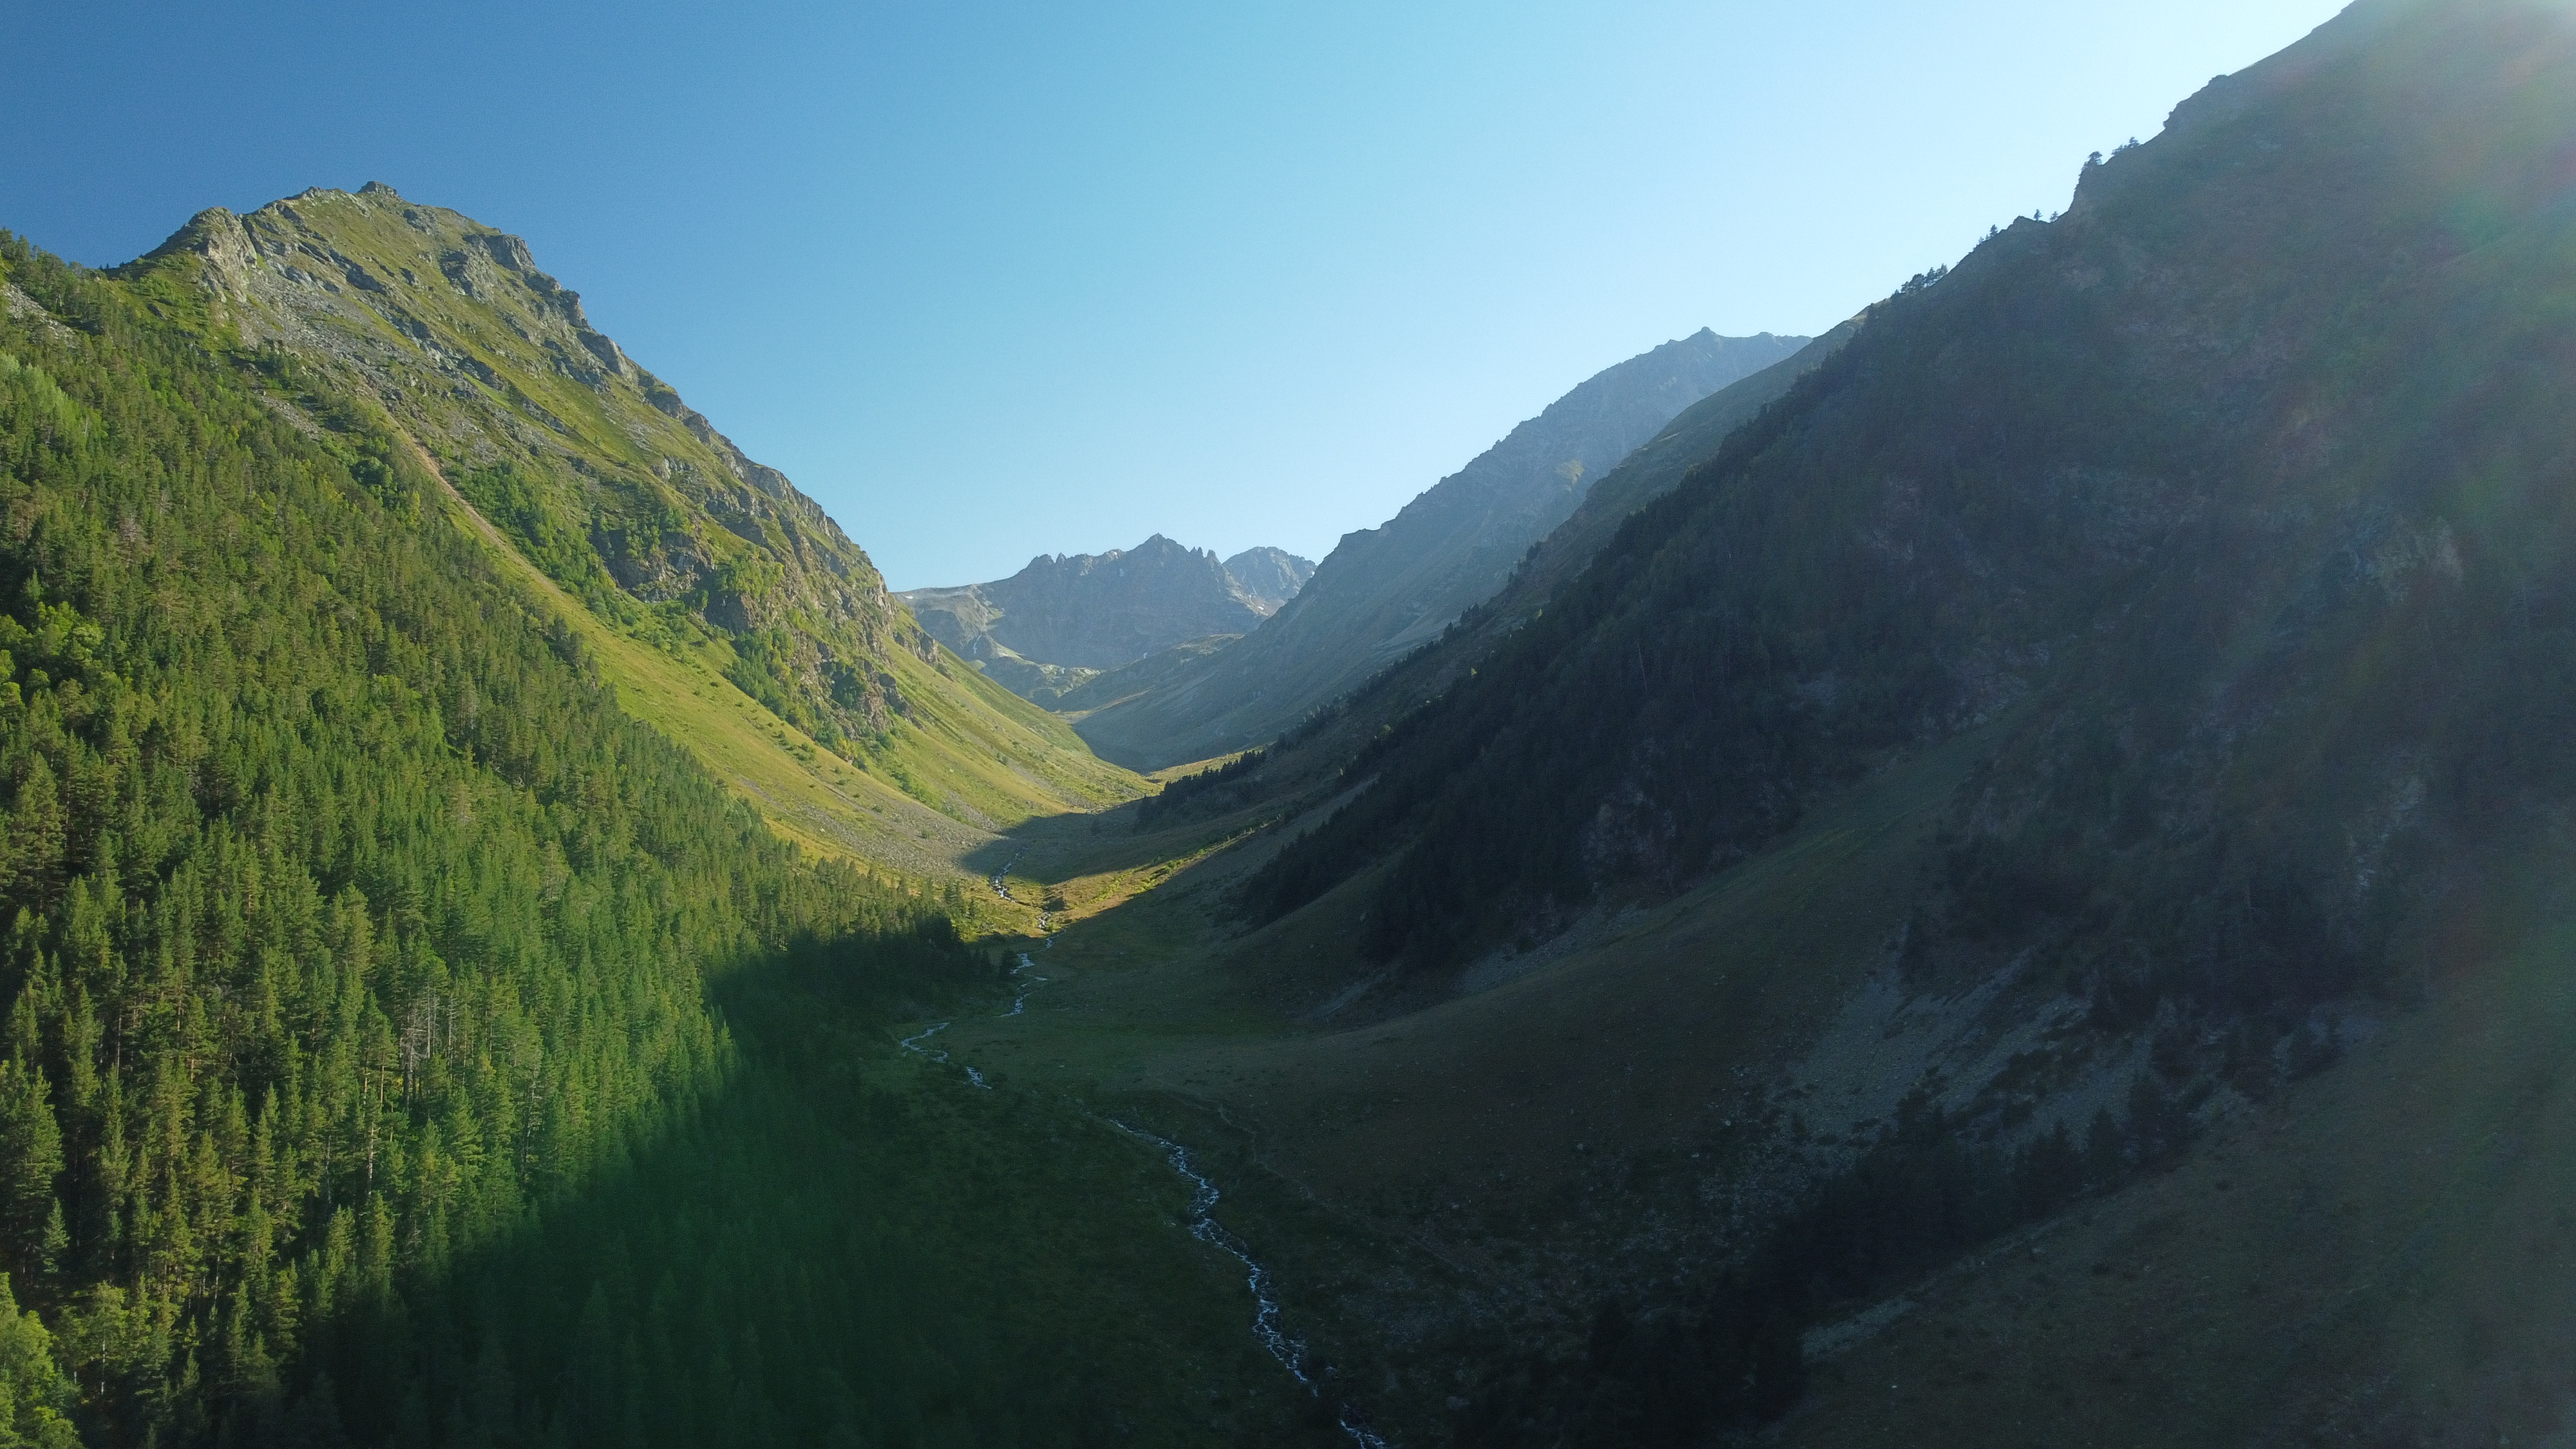
\includegraphics[width=0.7\linewidth]{../pics/DJI_0805}
	\caption{д.р. Кичкинакол Джалпаккольский}
	\label{fig:kichkinakol}
\end{figure}

После обеда в \alert{СКОЛЬКО?} проходим 2 км к оборудованной стоянке возле коша. Рядом местные жители собирают малину. Подумав немного и устроив разведку, поднимаемся ещё немного выше и встаём на место ночёвки на оборудованной стоянке возле дерева на небольшом разливе реки. Координаты м.н. N 43.35392\degree~E 41.96858\degree.
\begin{figure}[h]
	\centering
	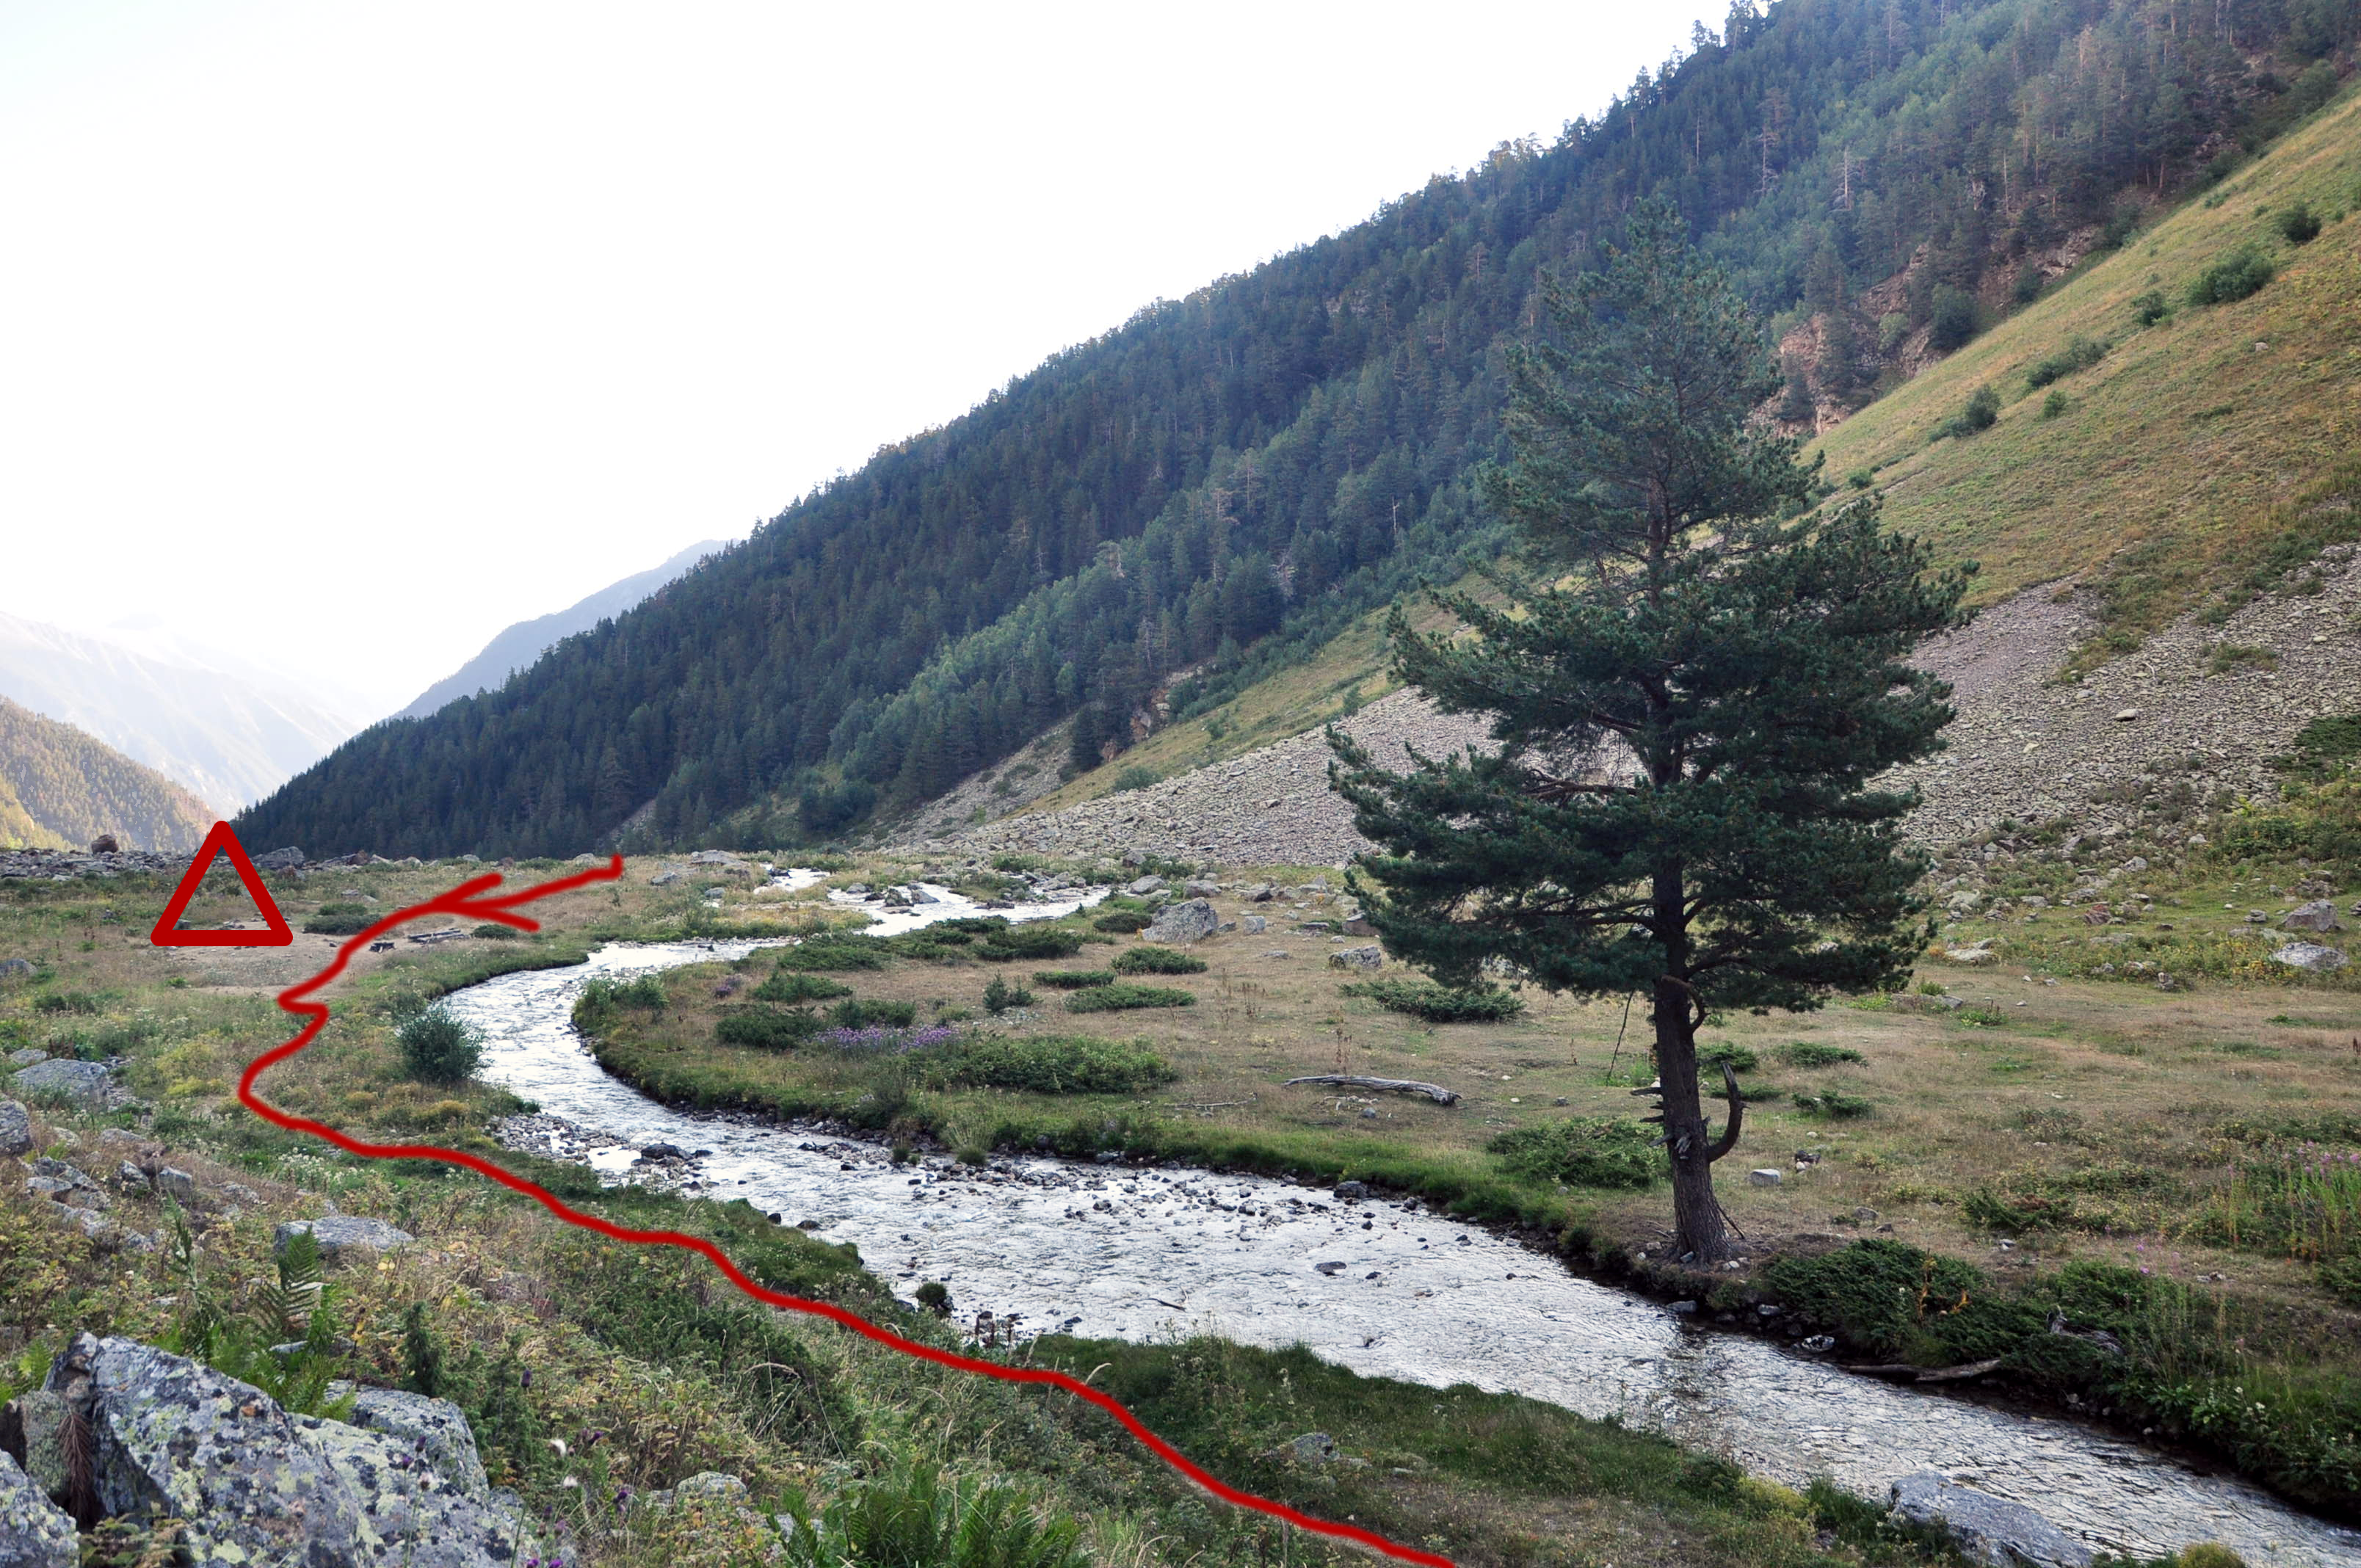
\includegraphics[width=0.7\linewidth]{../pics/camp_18}
	\caption{Место ночёвки 18-19.08}
	\label{fig:camp_18}
\end{figure}


\newpage